\documentclass[English]{article}
%^ Start of document
\usepackage{biblatex} %Imports biblatex package
\usepackage{graphicx} % Required for inserting images
\usepackage{authblk}
\usepackage[colorlinks=true, urlcolor=blue, linkcolor=red]{hyperref}
\usepackage{subfig}
\usepackage{float}
\usepackage{tabularx}
\usepackage{multirow}
\usepackage[paperheight=6in,
   paperwidth=5in,
   top=10mm,
   bottom=20mm,
   left=10mm,
   right=10mm]{geometry}
\usepackage{moresize}
\usepackage{tikz}
\usepackage{xcolor}
\usepackage{physics}
\usepackage{amssymb}
\usepackage{mathrsfs}
\usepackage{amsmath}
\usepackage{ragged2e}
\usepackage{comment}
\usepackage[paperheight=6in,
   paperwidth=5in,
   top=10mm,
   bottom=20mm,
   left=10mm,
   right=10mm]{geometry}
\addbibresource{bib.bib}
\begin{document}

\title{Atomic Models}

\author[1]{Zachary Tullier}
\affil[1]{University of Houston Clear Lake\\Physics Department\\Houston, Texas\\United States of America}
\date{April 19, 2024}

\maketitle

%\begin{abstract}   
%\end{abstract}


\section{Nuclear Fusion Overview and History}
Models of the atom began in the 5th century BC by ancient greek philosophers like Leucippus and Democritus. Even in this early stage the atomic models described small indivisible particles in motion that grouped together to form compounds. This model lasted over 2,000 years until John Dalton converted these ancient theories to the experimental foundation in chemistry. 

\section{Atomic Models}
In this section we will discuss the chronological list of atomic models up to the currently regarded description. 

\subsection{Atomic Model}
In 1808 John Dalton, a British scientist, categorized all the elements by mass and created a physical picture of how atoms exist and combine to eventually form compounds. In Dalton's theory the atoms were indivisible solid spheres. If two atoms were identical in properties then they were the same element. The different elements combined to form compounds. \cite{Dalton}
\begin{figure}[H]
    \centering
    {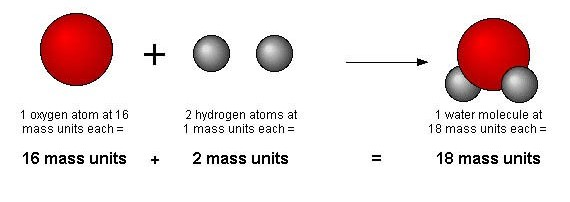
\includegraphics[width=0.4\textwidth]{Images/DaltonModel.jpg}\label{fig:f1}}
    \caption{Daltons Atomic Theory}
\end{figure}

\subsection{Plum Pudding Model}
In 1904 Joseph John Thomson, a British Physicist, further probed the atomic model by discovering a negatively charged particle. The electron shattered the ancient conception of a homogeneous atom. He adopted the "Plum-Pudding model" that placed electrons haphazardly in a positively charged "Soup". \cite{PlumPudding}.
\begin{figure}[H]
    \centering
    {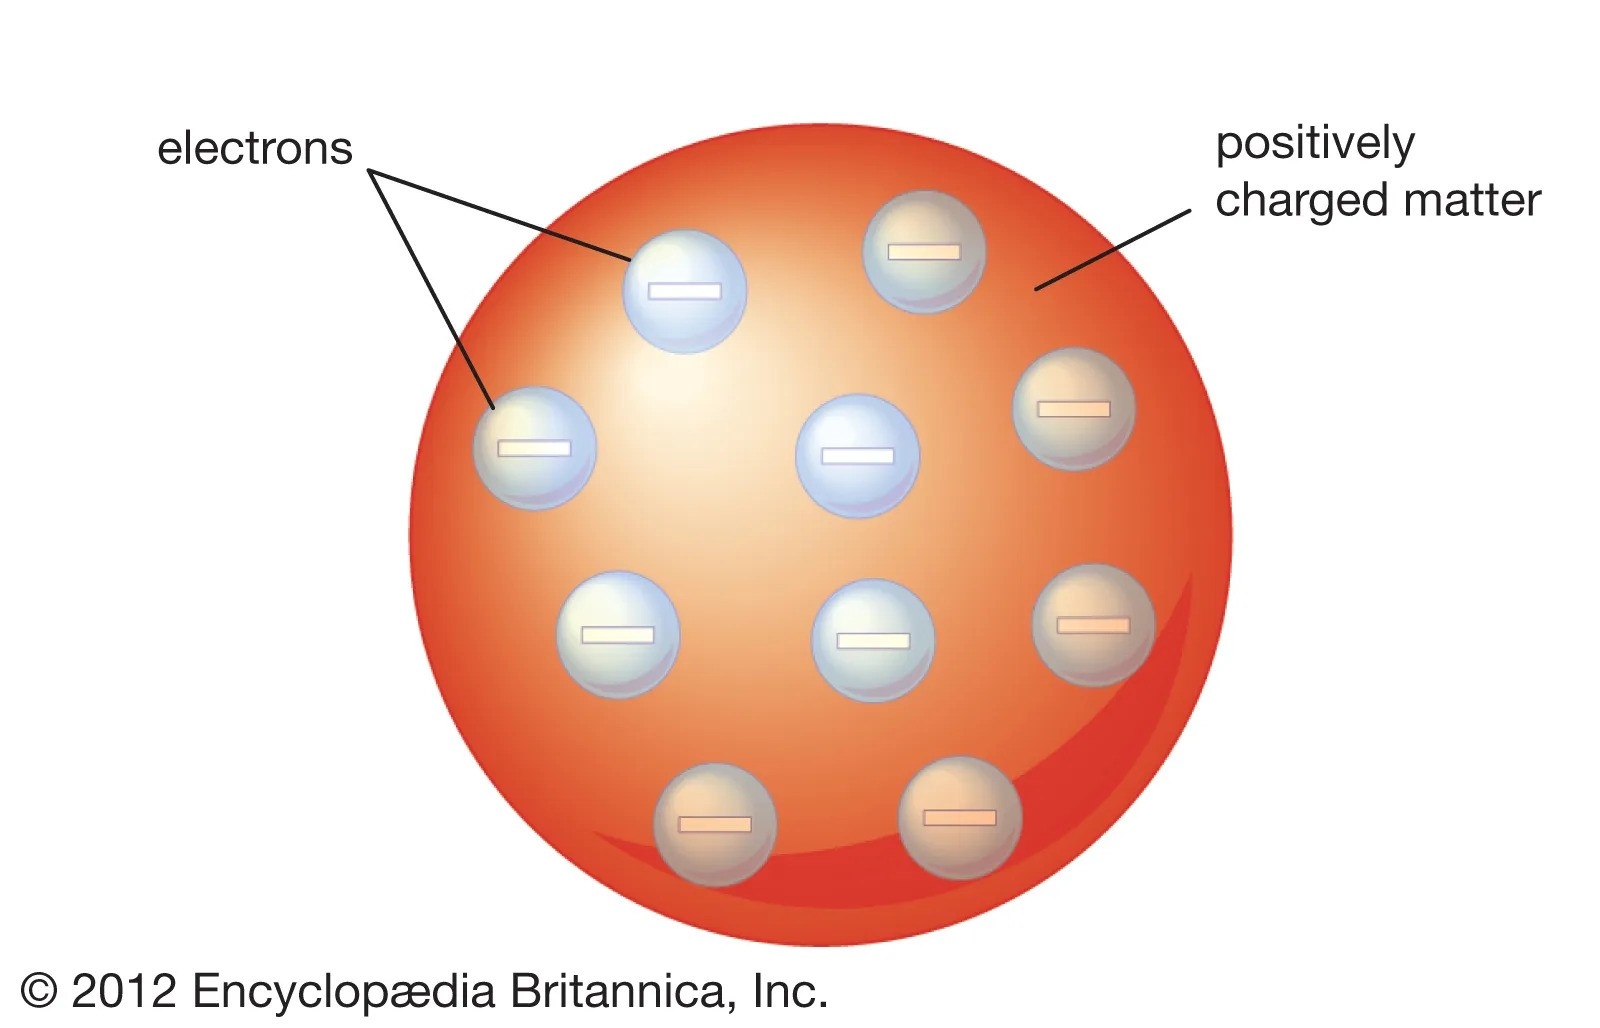
\includegraphics[width=0.4\textwidth]{Images/PlumPudding.jpg}\label{fig:f1}}
    \caption{Plum Pudding Atomic Model}
\end{figure}

\subsection{Rutherford Atomic Model}
In 1911 Earnest Rutherford, a New-Zealand Physicist, abolished the "Plum-Pudding" model and established a new model with experimental proof. Rutherford, along with a group of scientists, performed an experiment that focused helium nucleus particles at a gold foil sheet and mapped the collisions resulting particle spray. When a helium nucleus, or $\alpha$-particle, impacted the zinc sulfide screen it gave off a visible flash of light. Most of the $\alpha$-particles did not deviate much, but some bounced off into wide angles. This was evidence that there was an electric field around the central atom, matching Rutherford's predicted model \cite{Rutherford}. The model theorized that the positive charge of the atom was densely concentrated at the center with a negatively charged space around the edge, \cite{NucFund}. Rutherford's model resembled the shape of our solar system with the electrons orbiting the central positive mass. 
    \begin{figure}[H]
        \centering
        {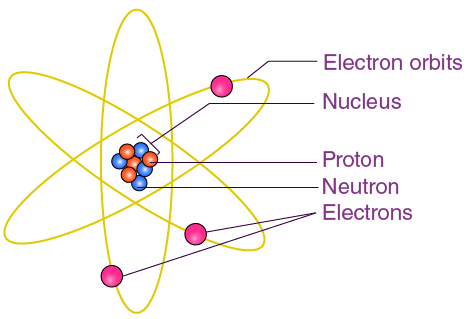
\includegraphics[width=0.4\textwidth]{Images/RutherfordModel.png}\label{fig:f1}}
        \caption{Rutherford Atomic Model}
    \end{figure}

\subsection{Bohr's Atomic Model}
In 1915 Neils Bohr, a Danish Physicist, combined Rutherford theories of orbital motion of electrons around a central nucleus with the quantum theory introduced by Max Planck \cite{Bohr}. Bohr's postulates are as follows: 
\begin{enumerate}
    \item "The atom consists of a dense nucleus of protons surrounded by equal number of electrons traveling in
discrete circular orbits (stationary states) at fixed distances
from the nucleus, retaining their motion under the influence
of the Coulomb force without emission of radiation."
This postulate allows the formation of the total orbital energy, $E=\frac{-Z_e^3}{4*\pi*\epsilon_0*r}$.
    \item "The different possible stationary states of a system
consisting of an electron rotating about a positive nucleus
are those for which the orbits are circles determined by the angular momentum L." 
This postulate allows the formation of the Bohr's Radius, $E=\frac{\hbar^2}{k_B*m*e^2}$, and the ground state energy, $E=\frac{-m*k^2*Z_e^2*e^4}{2*n^2*\hbar^2}$. Bohr's radius is an important parameter that predicts the most probable distance between the electron and nucleus of a hydrogen atom at its ground energy level.
    \item "Any emission or absorption of radiation will correspond to a transition between two stationary states."
This postulate allows the formation of the energy of absorption or emission, $h*\upsilon=E_f-E_i=E_1*(\frac{1}{n_f^2}-\frac{1}{n_i^2})$. This theory was the first to successfully account for the discrete energy levels measured in the laboratory for emission and absorption.
\end{enumerate}
    \begin{figure}[H]
        \centering
        {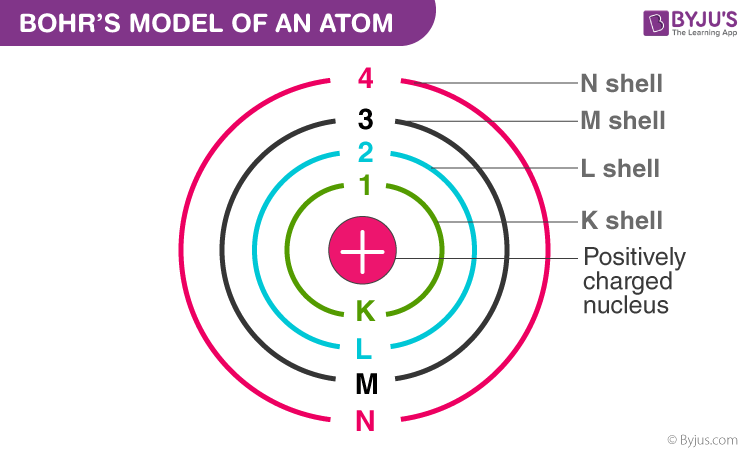
\includegraphics[width=0.4\textwidth]{Images/BohrModel.png}\label{fig:f1}}
        \caption{Bohr Atomic Model}
    \end{figure}

\subsection{Schrodinger Quantum Mechanical Model}
In 1926 Erwin Schrodinger, an Austrian-Irish Physicist, proposed that the electrons move around the nucleus in clouds of uncertainty \cite{PhysRev.28.1049}. This models still bears a similar shape to Bohr and Rutherford's models, but the electrons do not have fixed paths. This proposed that one could not be certain of the location or momentum of electrons orbiting a nucleus at the same time. No theory has surpasses Schrodinger's as a more accurate and repeatable explanation for the behavior of electrons around an atom. 
    \begin{figure}[H]
        \centering
        {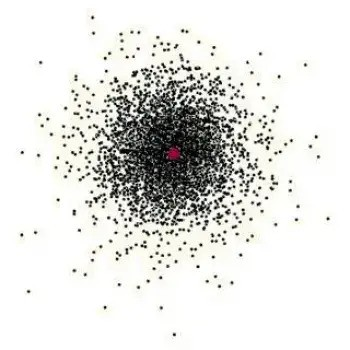
\includegraphics[width=0.4\textwidth]{Images/SchrodingerModel.jpg}\label{fig:f1}}
        \caption{Schrodinger Atomic Model}
    \end{figure}

\section{Nuclear Atomic Models}
In this section we will discuss the chronological list of nuclear atomic models up to the currently regarded description. 

\subsection{Liquid Drop Model}
In 1935, Carl Friedrich von Weizsacker, a German Physicist, introduced the Semi-Emperical Mass Formula \cite{Carl} which was based off of George Gamows Liquid Drop Model. While it was known to be an inadequate model for explaining all nuclear phenomena, it provided excellent estimates of the average properties of nuclei. The binding energy was formulated as:
\begin{gather*}
    E_b = a_V A - a_S A^{\frac{2}{3}} - a_C \frac{Z^2}{A^{\frac{1}{3}}} - a_A \frac{(A-2Z)^2}{A} \pm \delta(A,Z)\\
\end{gather*}
where Z is the number of protons in a nucleon and A is the sum of protons and neutrons in a nucleon. 
The "Volume Term" ($a_V A$) is the volume of an incompressible fluid caused by the strong force between the nucleons. Since the strong force has such a short range any given nucleon can only interact strongly with its neighbor and next nearest neighbor; therefore, it is proportional to A. 
The "Surface Term" ($a_S A^{\frac{2}{3}}$) is a correction to the "Volume Term"'s assumption that nucleons completely surround each other. In reality they have a pseudo surface tension when attracted together that counteracts the strong force. Geometrically this correction should be proportional to the surface area, i.e, $A^{\frac{2}{3}}$.
The "Coulomb Term" ($a_C \frac{Z^2}{A^{\frac{1}{3}}}$) describes the repulsion between the protons within a nucleus. Each proton has a positive electromagnetic charge that acts on all the other protons.
The "Asymmetry Term" ($a_A \frac{(A-2Z)^2}{A}$) is a correction for an non-equal distribution of protons an neutrons as a product of the Pauli Exclusion Principle. In heavier nuclei the neutrons are more numerous than the protons and electrically neutral. The Coulomb force between the protons is slightly negated by the strong force of the extra neutrons. 
The "Pairing Term" ($\delta(A,Z)$) is a correction for the effects of spin coupling. In a nucleon with an even number of protons and neutrons the spin of each particle is paired with its opposite; therefore, experiencing more stability. 
The coefficients of each term are experimentally measured. According to \cite{ModPhys}, the most recent and accepted formulation, the coefficients are measured to result in the following equation:
\begin{gather*}
    E_b = 15.76 A - 17.81 A^{\frac{2}{3}} - 0.711 \frac{Z^2}{A^{\frac{1}{3}}} - 23.7 \frac{(A-2Z)^2}{A} \pm 34 A^{\frac{-3}{4}}\\
\end{gather*}

    \begin{figure}[H]
        \centering
        \subfloat[Binding Energy Per nucleon vs number of protons of all elements and their known isotopes]{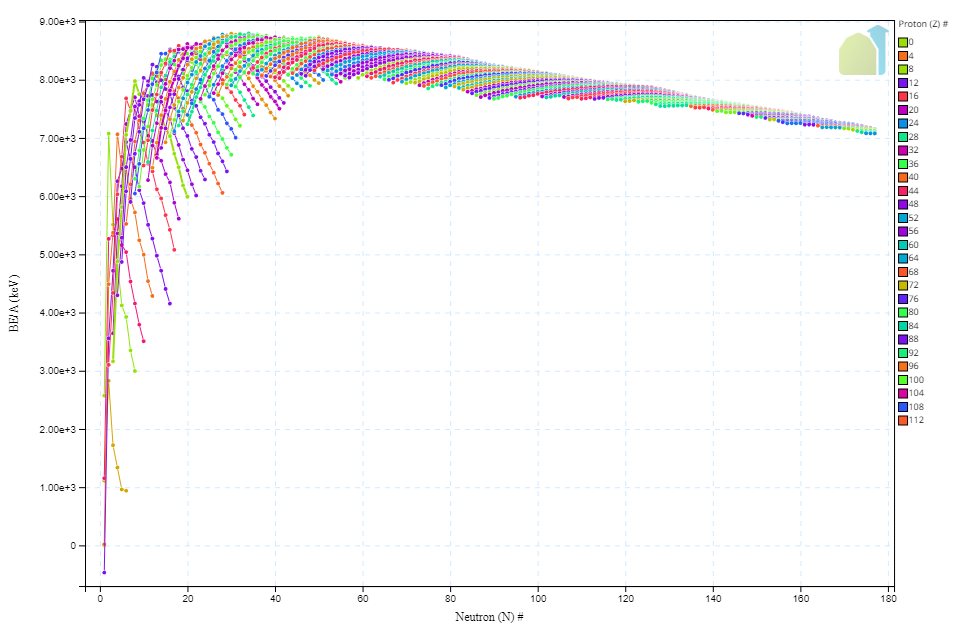
\includegraphics[width=0.4\textwidth]{Images/E_b_per_nucleon_Neut.png}\label{fig:f1}}
        \hfill
        \subfloat[Binding Energy Per nucleon vs number of neutrons of all elements and their known isotopes]{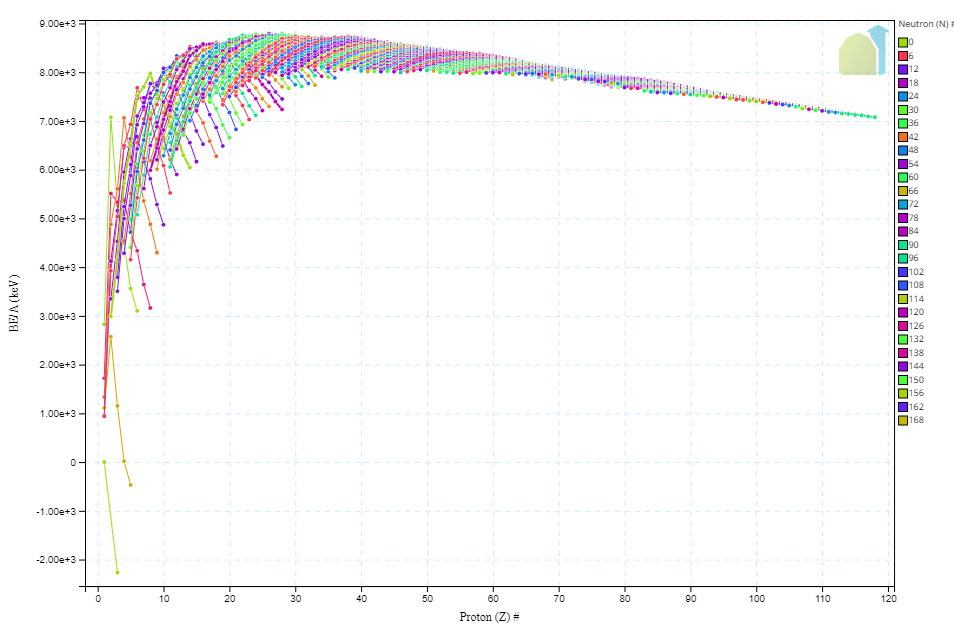
\includegraphics[width=0.4\textwidth]{Images/E_b_per_nucleon_Prot.png}\label{fig:f2}}
        \caption{Reference \cite{NuDat}}
    \end{figure}

\subsection{Nuclear Shell Model}
In 1932 Dmitri Ivanenko, a Ukrainian-Soviet Physicist, and E. Gapon proposed the Nuclear Shell model, but more practical advancements came in 1949 following independent work from several physicists. Most notably among those were the Nobel prize winners Maria Goeppert Mayer and J Hans D. Jensen. This model is analogous to the early atomic models that described the placement of electrons surrounding a nuclei, but this model describes the protons and neutrons as they are placed within the nuclei. The Shell model was originally formulated based on discrepancies found in the Semi-Empirical Mass Formula. It was found that there was a "Magic" number of protons and neutrons that created strongly bound states. The magic number observed over the range of nuclei are 
2, 8, 20, 28, 50, 82, and 126. "Doubly magic quantum nuclei" are nuclei where both the the number of protons and neutrons are both "Magic" numbers. These "Magic" numbers can be determined by approximating the model with a three-dimensional harmonic oscillator and a spin-orbit interaction or more accurately using the Wood-Saxon potential. 
 












\newpage
\printbibliography
\end{document}
